\zerar
\chapter{Geração de Viagens}
\label{cap:geracao}

Todos os métodos de solução do PDV (exatos ou heurísticos) exigem um mecanismo de geração 
explícita de viagens legais. Esses serão os objetos referentes às variáveis que desejamos otimizar. 

A geração pode ser eficientemente implementada através de um mecanismo de busca em uma rede de voos. 
O resultado da busca depende explicitamente das regras de trabalho impostas pelo contexto do
problema. As viagens geradas apresentam um custo também intimamente ligado ao contexto e ao 
objetivo que se deseja atingir. 

Neste capítulo apresentaremos mais detalhes sobre o procedimento de geração de viagens. Ao final,
será exibido um exemplo explícito.

%%%%%%%%%%%%%%%%%%%%%%%%%%%%%%%%%%%%%%%%%%%%%%%%%%%%%%%%%%%%%%%%%%%%%%%%%%%%%%%%%%%%%%%%%%%%%%%%%%%%

\section{Regras de Trabalho e Estrutura de Custo}
\label{sec:regras_e_custos}

É importante explicitar os tipos de restrições e a estrutura de custo envolvidos no problema, em 
especial no contexto brasileiro, já que há uma diferença significativa com relação aos contextos 
norte-americano e europeu, normalmente analisados na literatura.

No caso do PDV, a geração de uma viagem é regida por uma série de regras impostas pela Agência
Nacional de Aviação Civil (ANAC), além de restrições impostas por leis trabalhistas e acordos
contratuais. Uma viagem é dita legal se ela obedecer todas as regras impostas pela legislação em
questão. Abaixo apresenta-se valores típicos para as regras que regem a construção de uma viagem em
uma empresa de aviação regular do Brasil com voos de curto e médio alcance (veja a
Seção~\ref{sec:definicoes} para as defininições):

\begin{itemize}
	\item Duração máxima de uma jornada de trabalho: 11 horas;
	\item Número máximo de horas de voo em uma jornada: 9 horas e 30 minutos;
	\item Número máximo de pousos em uma jornada: 6 pousos;
	\item Descanso mínimo entre jornadas: 12 horas;
	\item Tamanho máximo de uma viagem: 6 dias;
	\item Tempo mínimo de conexão: 30 minutos;
	\item Tempo máximo de conexão: 4 horas;
	\item Número máximo de trocas de aeronave em uma jornada: 2 trocas;
	\item Tempo de {\it briefing}: 30 minutos fora de base e 45 minutos na base;
	\item Tempo de {\it debriefing}: 30 minutos.
\end{itemize}

O custo de uma viagem está associado à produtividade mais os custos referentes à estadia do 
tripulante quando esse precisar pernoitar fora da base, além das diárias de alimentação. Uma 
expressão típica para calcular o custo $c_p$ de uma viagem $p$ é dada por
%
\begin{equation} \label{eq:custov} 
	c_p = \sum_{d \in D_p} c_d \, , \;\;
	c_d = \alpha_0 \left[t_d - \left(tp_d - \sum_{i \in I_d} t_i\right)\right] + cp_d \ev
\end{equation} 
%
onde
%
\begin{itemize}
	\item[$D_p$:] conjunto de jornadas que constituem a viagem $p$;
	\item[$c_d$:] custo da jornada $d$;
	\item[$\alpha_0$:] custo da hora de trabalho do tripulante;
	\item[$t_d$:] duração da jornada $d$ (em horas);	
	\item[$tp_d$:] tempo de preparação ({\it briefing} mais {\it debriefing}) usado na jornada $d$;
	\item[$I_d$:] conjunto de etapas que compõe a jornada $d$;
	\item[$t_i$:] duração da etapa $i$, incluindo o tempo mínimo de conexão;
	\item[$cp_d$:] custo do pernoite mais diárias de alimentação da jornada $d$.
\end{itemize}
%
Note que a expressão que multiplica $\alpha_0$ em (\ref{eq:custov}) representa o tempo que o
tripulante passou trabalhando sem estar voando, portanto representa uma medida de produtividade.
Quanto mais cara a viagem, menor foi a produtividade do tripulante.

A estrutura descrita acima se refere a um modelo padrão para companhias aéreas brasileiras.
Fora do Brasil, entretanto, a estrutura do custos pode ser diferente. Nos Estados Unidos, por 
exemplo, o custo de uma viagem é dado por uma função não-linear de diferentes custos. 
Especificamente, o custo de uma viagem $p$ é dado por
%
\begin{equation*}
	c_p = \max\left\{\sum_{d \in D_p} MIN\_GRT_d \ev \sum_{d \in D_p} FLY\_TIME_d \ev 
	TIME\_AWAY_p \right\} \ev
\end{equation*}
%
onde $MIN\_GRT_d$ é o mínimo de garantia oferecido ao tripulante ao voar a jornada $d$, 
$FLY\_TIME_d$ é o tempo de voo da jornada $d$ (pode ser multiplicado por algum fator) e
$TIME\_AWAY_p$ é o tempo total que o tripulante passa fora de sua base na viagem $p$ (também pode
ser multiplicado por algum fator). Observe assim, que nesse modelo, o custo de cada etapa depende da
viagem em ela está incluída.

%%%%%%%%%%%%%%%%%%%%%%%%%%%%%%%%%%%%%%%%%%%%%%%%%%%%%%%%%%%%%%%%%%%%%%%%%%%%%%%%%%%%%%%%%%%%%%%%%%%%

\section{Gerador de Viagens}
\label{sec:gerador_viagens}

O primeiro passo em direção à solução do PDV consiste na implementação de um gerador de viagens 
eficiente que seja capaz de produzir um grande número de viagens legais em pouco tempo. Como já
mencionamos, os métodos de resolução de (\ref{eq:sppv}) baseiam-se no conceito de 
``gerar-e-otimizar'', e já que as rotinas de otimização estão normalmente prontas em pacotes 
fechados, a parte de geração é de grande importância.

Uma viagem pode ser vista como um caminho especial em um grafo estruturado. Esse grafo é chamado de
\emph{rede de voos} e será detalhado a seguir. 

As etapas na rede de voos podem ser representadas como nós ou arcos. Escolhemos a representação em
termos de arcos. Os nós da rede representam as saídas e chegadas de cada etapa, bem como uma fonte
$s$ e um sorvedouro $t$. Existe um arco representando cada etapa da malha de voos. Para o problema
diário, replicamos cada arco quantas vezes for o número máximo de dias permitido em um viagem. O
conjunto de arcos será denotado por $\calA$.

O nó fonte é ligado ao nó de saída de cada etapa que se origina em uma base específica. O nó de
chegada de cada etapa que termina nessa base é ligado ao sorvedouro. Existem ainda arcos
representando conexões legais entre etapas. Um par de etapas terá um arco de conexão entre eles se
o aeroporto de chegada do primeiro corresponder ao aeroporto de saída do segundo, e o intervalo de
tempo entre a chegada e a saída estiver for uma conexão legal de uma jornada, 
ou descanso regular entre jornadas. 

É fácil notar que toda viagem legal é representada por um caminho $s-t$ na rede de voos. Porém,
existem caminhos $s-t$ que não representam viagens legais pois podem desrespeitar alguma regra de
trabalho, embora as conexões possíveis sejam legais. A estrutura da rede garante que não seja feita
nenhuma conexão entre duas etapas que não tenham suas respectivos destino e origem coincidentes no
espaço e no tempo. Entretanto, não garante, por exemplo, que o número máximo de horas de voo
permitido em uma jornada seja excedido. 

O gerador de viagens funciona aplicando um algoritmo de busca em profundidade à rede de voos. O
algoritmo inicia-se no nó de origem $s$ e explora todas a conexões viáveis $(i, j) \in \calA$, até
retroceder. O processo de busca em profundidade controla a viabilidade das viagens, levando em conta
a duração máxima das jornadas e limites de horas de voo e de pousos, etc (ou seja, verifica as 
regras de trabalho ao atravessar cada aresta).

%%%%%%%%%%%%%%%%%%%%%%%%%%%%%%%%%%%%%%%%%%%%%%%%%%%%%%%%%%%%%%%%%%%%%%%%%%%%%%%%%%%%%%%%%%%%%%%%%%%%

\section{Exemplo}
\label{sec:exemplo}

A tabela abaixo mostra um conjunto fictício (para fins de ilustração) de 7 etapas operadas 
diariamente entre as localidades A, B, C e D. O exemplo é adaptado de~\cite{barnhart03}. 

\begin{table}[ht]
	\begin{center}
		\begin{tabular}{ccccc}
			{\bf \# Etapa} & {\bf Origem} & {\bf Destino} & {\bf Saída} & {\bf Chegada} \\ \hline
			1 & A & B & 08:00 & 09:00 \\
			2 & B & C & 10:00 & 11:00 \\
			3 & C & D & 13:00 & 14:00 \\
			4 & C & A & 15:00 & 16:00 \\
			5 & D & A & 15:00 & 16:00 \\
			6 & A & B & 17:00 & 18:00 \\
			7 & B & C & 11:00 & 12:00 \\
		\end{tabular}
	\end{center}
\end{table}

A rede de voos (parcial) para uma base contratual A é ilustrado na Figura~\ref{fig:rede}, onde são
apresentadas algumas das conexões legais possíveis para clareza do desenho. O caminho vermelho
na figura representa uma viagem legal com dois dias de duração. 

A partir da rede apresentada, montamos as seguintes jornadas válidas (os números representam os
números das etapas)
%
\begin{eqnarray*}
	&& D_1 = \{1\} \ev \hsp D_2 = \{2\} \ev \hsp D_3 = \{3\} \ev \hsp D_4 = \{4\} \\
	&& D_5 = \{5\} \ev \hsp D_6 = \{6\} \ev \hsp D_7 = \{7\} \ev \hsp D_8 = \{1, 2\} \\
	&& D_9 = \{1, 7 ,3\} \ev \hsp D_{10} = \{2, 3\} \ep 
\end{eqnarray*}

Assumindo que as localidades A, B e D sejam bases contratuais, geramos seis viagens, que podem ser
expressas em termos das jornadas como 
%
\begin{eqnarray*}
	&& P_1 = \{D_4, D_8\} \ev \hsp P_2 = \{D_9, D_5\} \ev \hsp P_3 = \{D_5, D_6, D_{10}\} \\
	&& P_4 = \{D_4, D_6, D_7\} \ev \hsp P_5 = \{D_1, D_7, D_4\} \ev \hsp P_6 = \{D_5, D_7, D_9\} \ep 
\end{eqnarray*}

Note que a viagem $P_6$ cobre a etapa $7$ duas vezes, então ela não é válida e deve ser 
desconsiderada. Supondo que os custos associados as viagens sejam $c_1 = c_2 = c_3 = c_4 = 4$ e
$c_5 = 5$, a partir de (\ref{eq:sppv}) obtemos o seguinte problema ($x_i \in \{0, 1\}$, 
$i=1, \ldots, 5$):
%
\begin{equation*}
	\begin{array}{lllllllllllll}
		\text{min} & 4x_1 & + & 4x_2 & + & 4x_3 & + & 4x_4 & + & 5 x_5 & & & \vsp \\ 
		& x_1 & + & x_2 & & & & & + & x_5 & = & 1 & \text{(etapa 1)} \vsp \\
		& x_1 & & & + & x_3 & & & & & = & 1 & \text{(etapa 2)} \vsp \\
		& & & x_2 & + & x_3 & & & & & = & 1 & \text{(etapa 3)} \vsp \\
		& x_1 & & & & & + & x_4 & + & x_5 & = & 1 & \text{(etapa 4)} \vsp \\
		& & & x_2 & + & x_3 & & & & & = & 1 & \text{(etapa 5)} \vsp \\
		& & & & & x_3 & + & x_4 & & & = & 1 & \text{(etapa 6)} \vsp \\
		& & & x_2 & & & + & x_4 & + & x_5 & = & 1 & \text{(etapa 7)}
	\end{array}
\end{equation*}

Se pelo menos 3 horas e no máximo 6 horas estejam disponíveis nas bases A e D, e no máximo 5 horas 
na base C, então as restrições de bases (\ref{eq:bases}) são
%
\begin{equation*}
	\begin{array}{ll}
		3 \leq 4 x_2 + 3 x_5 \leq 6 & \text{(base A)} \vsp \\
		0 \leq 3 x_1 + 3 x_4 \leq 5 & \text{(base C)} \vsp \\
		3 \leq 4 x_3 \leq 6 & \text{(base D)}
	\end{array}
\end{equation*}

A solução ótima para o problema formulado usa as viagens 3 e 5 ($x_3 = x_5 = 1$, 
$x_1 = x_2 = x_4 =  0$) e tem um custo total igual à 9. Por se tratar de um problema pequeno, a
resolução do mesmo pode ser obtido por qualquer pacote de otimização linear.

\begin{figure}[htbp]
	\begin{center}
		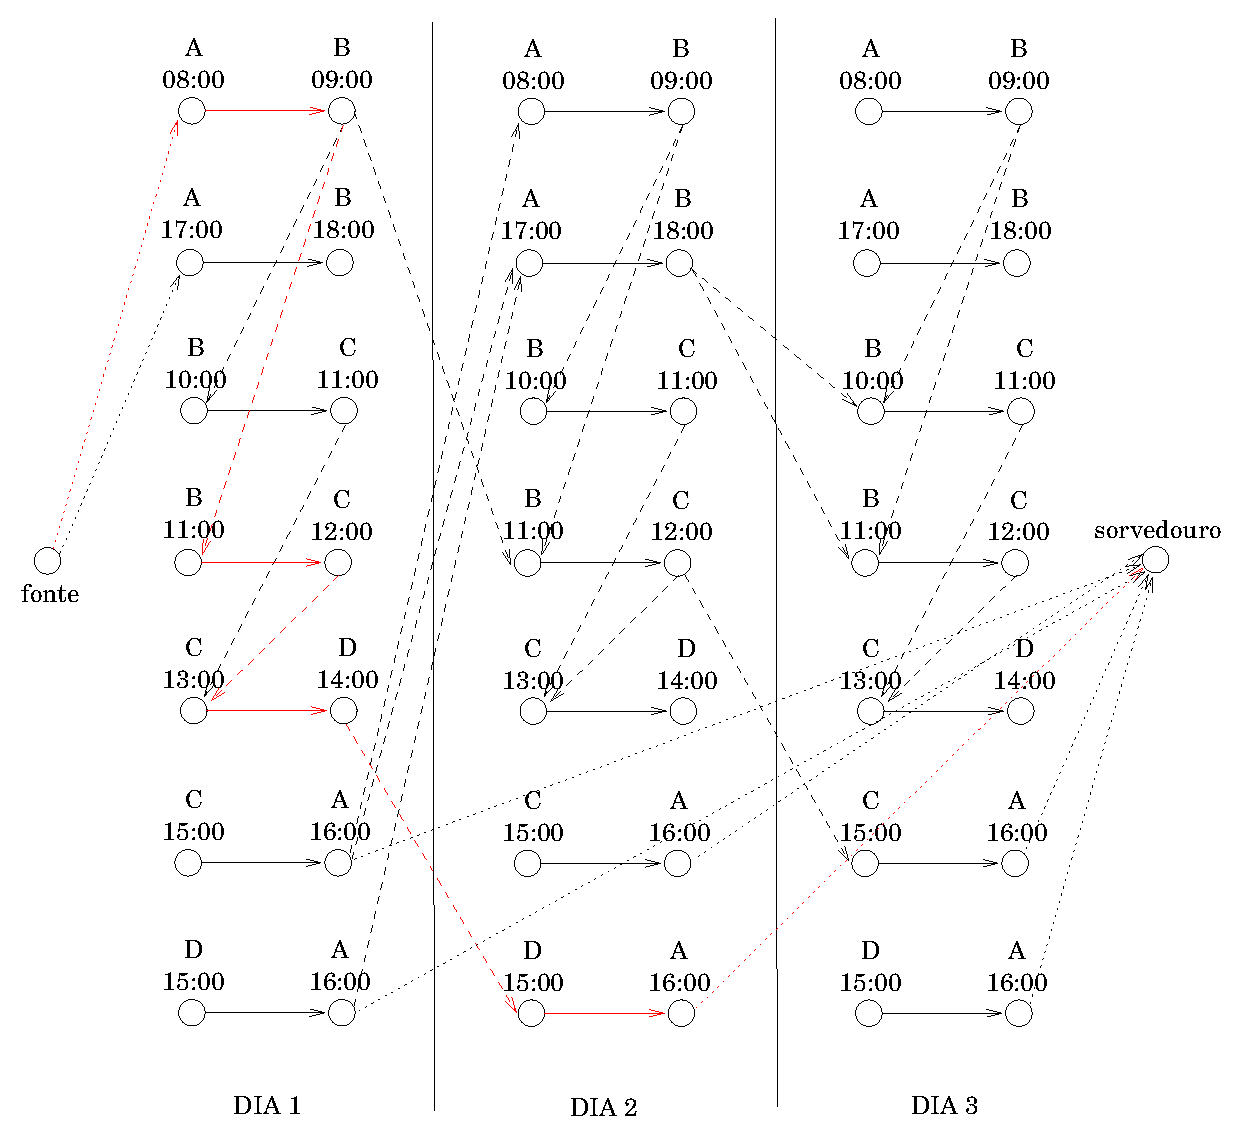
\includegraphics[scale=0.80]{fig/rede.eps}
		\caption{Rede de voos referente às 7 etapas do exemplo ilustrativo. Consirou-se viagens de no 
		máximo 3 dias, por isso os nós são replicados três vezes para o problema diário. A base dos 
		tripulantes considerada foi a localidade A, dando origem as ligações da fonte e do sorvedouro.
		Arcos tracejados representam conexões legais entre localidades. O caminho em vermelho representa
		uma das viagens possíveis.}
		\label{fig:rede}
	\end{center}
\end{figure}

%%%%%%%%%%%%%%%%%%%%%%%%%%%%%%%%%%%%%%%%%%%%%%%%%%%%%%%%%%%%%%%%%%%%%%%%%%%%%%%%%%%%%%%%%%%%%%%%%%%%
